\clearpage % clear the prior chapter's page

\chapter{Analysis and modeling applications of DEER data}\label{ch:intro_deer}
%\vspace{-7mm}

\bigskip

This Chapter presents an overview of the methods available to analyze \gls{deer} data and apply the resulting distance distributions to model protein structures. Particular attention is paid to interpreting these data using Tikhonov regularization and Gaussian mixture models. Distributions converted from the time domain using these methods can then be used to guide structural modeling. Commonly used strategies for integrating these experimental data as restraints are discussed. This Chapter concludes by speculating on how the analysis of \gls{deer} data and its application for modeling protein structures can be coupled.

\section{Introduction}

Among the tools available to the field of structural biology, \gls{deer} spectroscopy is uniquely suited to monitor the dynamic properties of proteins \citep*{Hubbell2000, Jeschke2012, Mchaourab2011}. \Gls{deer}, also called PELDOR, measures nanometer-scale distance distributions between two paramagnetic probes attached to the protein's surface. By resolving and reporting full distributions, rather than just average distance values, \gls{deer} can reveal conformational heterogeneity and intermediate states that may be inaccessible to crystallography and \gls{cryoem}. The contribution of this technique to the derivation of mechanistic inferences has been bolstered in recent years by its integration with computational modeling \citep*{Jeschke2018a}. Distributing experimental measurements throughout the structure of a protein allows qualitative conclusions to be synthesized into quantitative structural models. Computational modeling allows one-dimensional distance data to be interpreted in the context of a three-dimensional structural models, thus facilitating further hypothesis testing.

Nonetheless, computational modeling and \gls{deer} spectroscopy are each areas of research under active development. Their integration in the literature is highly nonstandard, with customized protocols often being used on a case-by-case basis. As will become clear in this chapter, best practices are far from established. Individually, each method provides opportunities to make unwarranted inferences; in tandem, they present a risk of overfitting the data and arriving at spurious conclusions. Perhaps as a result, most studies employ the data conservatively and deliberately underleverage some of the \gls{deer} technique's advantages, such as its ability to reveal minor populations. This hinders the development of one’s understanding of a protein’s structural dynamics. Nonetheless, recent methodological advancements in both \gls{deer} data analysis and macromolecular modeling promise to mitigate this possibility.

This chapter discusses the analysis of four-pulse \gls{deer} data \citep*{Pannier2000} and its interpretation by structural modeling. We focus our attention on the common experimental scenario where proteins are labeled with two flexible spin-$\frac{1}{2}$ nitroxide probes per macromolecule and flash-frozen prior to measurement. Our discussion is limited with respect to more exotic applications, include alternative pulse sequences \citep*{Borbat2013, Breitgoff2017, Mentink-Vigier2013, Spindler2015}, labeling with lanthanide ions \citep*{Giannoulis2019, Matalon2013, Potapov2010, Yagi2011} or noncanonical amino acids \citep*{Braun2019, Schmidt2015, Schmidt2015a}, deliberate introduction of orientation effects \citep*{Bowen2018, Endeward2009, Marko2013}, specialized sample preparation conditions for long-distance measurements \citep*{ElMkami2015, Schmidt2016}, and interpretation of measurements performed at room temperature \citep*{Graenz2018, Kuzhelev2016, Meyer2015} or in cells \citep*{Azarkh2019, Joseph2016, Singewald2019, Yang2019}. The scope of this chapter nonetheless encompasses the vast majority of integrative modeling studies. That being said, the \gls{deer} technique is certain to continue evolving; it is not difficult to envision room-temperature experiments capable of in-cell measurements in proteins with many conserved cysteines.

\section{Analysis of DEER data}\label{sec:deerintro_deeranalysis}

\subsection{Composition of the DEER signal}

Pulse \gls{epr} methods measure the amplitude of spin echoes caused by the successive application of microwave-frequency pulses to samples containing unpaired electrons in the presence of an external magnetic field \citep*{Milov1998, Milov1983}. The signal obtained from a four-pulse \gls{deer} experiment reflects time-dependent spin-spin coupling within a macromolecule ($S(t)$) and across macromolecules ($B(t)$):

\begin{equation}
    \frac{ V \left( t \right)}{ V_0 } = B \left( t \right) * \left( 1 - \lambda \left( 1 - S \left( t \right) \right) \right) + \epsilon
    \label{eq:deerintro_total}
\end{equation}

Here $\frac{V \left( t \right)}{ V_0 }$ denotes the normalized signal amplitude and $\epsilon$ is normally distributed experimental noise in the signal \citep*{Edwards2016}. The modulation depth $\lambda$ reports the spin inversion efficiency and is also affected by the parameters of the \gls{deer} experiment. The background coupling signal is most commonly modeled using the following stretched exponential function $B\left( t \right) = \exp \left( -k | t|^\frac{d}{3} \right)$ and relates the background spin concentration $k$ and the intermolecular coupling dimensionality $d$ (with $d$=3 except under circumstances where, for example, membrane proteins are reconstituted into lipid environments). Alternative background functions can be used to account for an excluded volume effect observed when the size of the molecule under study forbids short-distance intermolecular coupling \citep*{Kattnig2013}.

Ultimately the spectroscopist seeks to isolate and extract the distance information encoded by $S(t)$. Although the background coupling parameters $k$, $d$, and $\lambda$ report biologically meaningful information \citep*{Jeschke2004}, they are frequently treated as nuisance parameters during the analysis of \gls{deer} data. Nevertheless, their identification is critical to the accurate recovery of experimental distance data, and failure to disentangle $S(t)$ from background contributions to the signal can corrupt the resulting distance distribution by, for example, introducing spurious long-distance peaks \citep*{Jeschke2006}.

\subsection{Intramolecular contributions to the experimental signal}

The isolation of $S(t)$ and its conversion into a distance distribution $P(r)$ is at the heart of substantial research and methods development. The two are related by the following kernel function:

\begin{equation}
    S \left( t \right) = \int_{0}^{\infty} K \left( t, r \right) P \left( r \right) \mathup{d}r
\end{equation}

\begin{equation}
    K \left( t, r \right) = \int_{0}^{\frac{ \pi}{2}} \sin \theta \cos \left( \frac{ \left( 1 - 3 \cos^{2} \theta \right) \mu_0 \mu_{\mathup{B}}^{2} g_{\mathup{X}}^{2} t }{ 4 \pi \hslash r^{3} }  \right) \mathup{d} \theta
\label{eq:deerintro_kernel}
\end{equation}

Here $μ_B$ is the Bohr magneton, $μ_0$ is the vacuum permeability constant, $g$ is the electron g-factor, $r$ is the interspin distance in nanometers, $t$ is the timing of the third pulse in microseconds, and $\theta$ is the angle between the interspin vector and the bulk magnetization vector (we emphasize the distinction of $\theta$ from $\vartheta$, which denotes the parameters of a model and is used in Equations \ref{eq:deerintro_fitmodel}, \ref{eq:rosettadeer_kernel}, \ref{eq:aicc}, \ref{eq:multilateration_accept}, \ref{eq:multilateration_loglikelihood}, and \ref{eq:multilateration_kernel} below). Detailed derivations of \ref{eq:deerintro_kernel} are available \citep*{Worswick2018}. In practice, the \gls{deer} signal $S$ and distance distribution $P$ are discretized into time points and distance bins, respectively. The relationship between the intramolecular component of the signal $S$ and the probability distribution $P$ to $K$ can be denoted by the matrix-vector multiplication $S=KP$. Unfortunately, $P$ cannot be obtained by matrix inversion, as $K$ is close to singular \citep*{Edwards2016, FabregasIbanez2019}; consequently, the problem is ill-posed. The resultant distributions are spiky, unstable, overly sensitive to the noise in the data, and almost certainly not representative of actual distance values between unpaired electrons in the sample. Their shapes contrast with our expectation of smoothness from distributions of distances between flexible nitroxide probes attached to flexible macromolecules. In short, obtaining distributions using ordinary least squares is not an option.

\begin{wraptable}{r}{0.4\textwidth}
\scriptsize
\renewcommand{\tabcolsep}{0.09cm}
\centering
\caption[Commonly used methods for analyzing DEER data.]{Commonly used methods for analyzing DEER data.}

\newcolumntype{Y}{>{\raggedright\arraybackslash}X}

\begin{center}
\begin{tabular}{l r}
\toprule \\
\textbf{Method} & \textbf{Reference} \\
\midrule \\
Pake transformation &	\citep*{Jeschke2002} \\
Tikhonov regularization &	\citep*{Chiang2005, Jeschke2004} \\
Osher’s Bregman iterative regularization &	\citep*{FabregasIbanez2019} \\
Integral Mellin Transform &	\citep*{Matveeva2017} \\
Neural networks &	\citep*{Worswick2018} \\
Monte Carlo &	\citep*{Dzuba2016} \\
Wavelet denoising &	\citep*{Srivastava2016} \\
Maximum entropy/Tikhonov &	\citep*{Chiang2005a} \\
Sum-of-gaussians model-based fitting & \citep*{Brandon2012, Stein2015} \\
\bottomrule \\
\end{tabular} 
\end{center}




\label{tab:deerintro_methods}
\end{wraptable}

Thus, the analysis of \gls{deer} data must overcome two problems. First, the background component of the signal must be correctly identified, and second, the intramolecular component must be interpreted into distance data without overfitting noise in the signal. Both problems, particularly the latter, are subjects of active research and have been addressed using a wide range of mathematical strategies. Several approaches have been developed over the past two decades and are listed in Table \ref{tab:deerintro_methods} and shown in Figure \ref{fig:deerintro_methods}. For brevity, the following discussion is limited to Tikhonov regularization and model-based fitting, which are perhaps the two most widely used approaches in the literature. We note that for high-quality data containing an unambiguous background coupling component and a high \gls{snr}, the distributions reported by these methods are nearly identical. Methodological idiosyncrasies become more pronounced as the fidelity of the experiment signal decreases and the intramolecular coupling component $S(t)$ becomes difficult to isolate.

\begin{figure}[h]
\centering
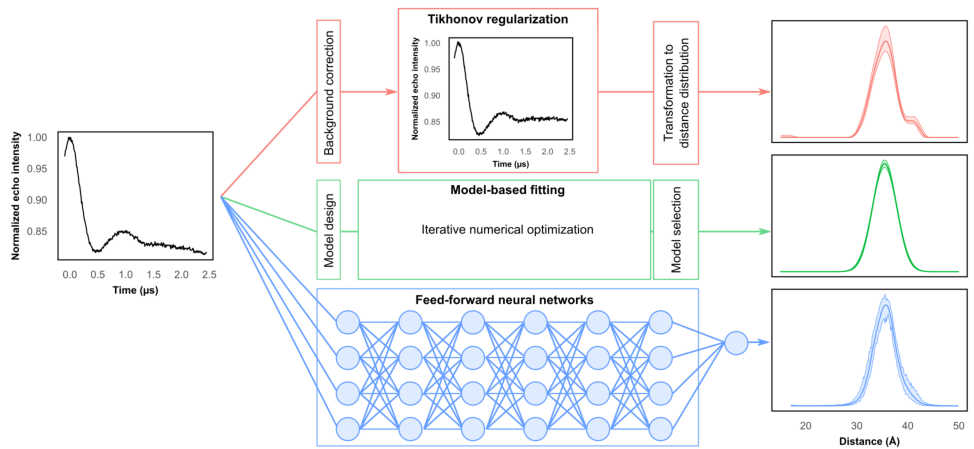
\includegraphics[width=6.5in]{deerintro_methods.pdf}
 \caption[Commonly used methods for analyzing DEER data.]{Commonly used methods for analyzing DEER data.}
\label{fig:deerintro_methods}
\end{figure}

\subsection{Tikhonov regularization}

A widely used approach to stabilizing ill-posed linear problems is to include a penalty term, which is denoted by $L$ and is specific for the problem at hand, that quantifies our expectations of what a reasonable solution should look like. Tikhonov regularization provides a general framework for integrating this penalty term into ordinary least-squares problems \citep*{Tikhonov1963}. The general strategy calculates the optimal probability distribution $\hat{P}$̂ by minimization of both the sum of squared residuals $\norm{KP-S}^2$ and the penalty term $\norm{LP}^2$:

\begin{equation}
    \hat{P}=\underset{P≥0}{\operatorname{\arg \min}} \left\{ \norm{KP-S}^2 + \alpha^2 \norm{LP}^2 \right\}
\end{equation}

Ultimately, the goal of this approach is to generate a smooth distribution with gradual changes in amplitudes between distances fractions of an angstrom apart. For example, it seems unreasonable to expect the peak of a distribution to be at \SI{34.1}{\angstrom} if the probability at \SI{34.0}{\angstrom} is zero. An effective penalty term would therefore restrain the derivative of the distribution, rather than the distribution itself. For this reason, the most widely used matrix penalizes changes in the second derivative \citep*{Edwards2018, FabregasIbanez2019, Jeschke2004}:

\begin{equation}
    L_2 = \begin{bmatrix} 
    1 & -2 & 1 & & & 0 \\
     & 1 & -2 & 1 & & \\
     & & \ddots & \ddots & \ddots & \\
     0 & & & 1 & -2 & 1 \\
    \end{bmatrix}
\end{equation}

This applies the smoothness constraint uniformly throughout the distribution, thus avoiding the spikiness observed by ordinary least-squares fitting. The weight of this term, relative to that of the least-squares term, is determined by the regularization parameter $\alpha$, which does not reflect an experimental variable and is only used to stabilize the probability distribution in solution. In general, lower-quality data require more regularization, and thus larger $\alpha$ values. For any given value of $\alpha$, one of several iterative non-negative least-squares algorithms can be used to obtain an optimal solution \citep*{Bro1997, Lawson1974}.

Not surprisingly, determining the most appropriate value for $\alpha$ is critical to the accurate recovery of distance data. It should be high enough to avoid overfitting noise in the time domain, but no higher than necessary to minimize information loss in the distance domain. Prior to 2018, the most common approach for selecting a value for $\alpha$ was to use an L-curve, in which the distribution is calculated using many values, and the resulting logarithm of the least-squares term of each fit is plotted as a function of the logarithm of the penalty term \citep*{Chiang2005, Jeschke2004}. However, a recent benchmark did not find the widespread practice of selecting the value of $\alpha$ from the “elbow” of this plot to be particularly effective \citep*{Edwards2018}. Instead, the authors proposed using either the \gls{aic} \citep*{Akaike1973} or generalized cross-validation \citep*{Lukas2006}, and since then the use of the former has become standard practice \citep*{FabregasIbanez2020a}. A follow-up study by Fábregas-Ibáñez and Jeschke found that iterative regularization methods can further improve the quality of distributions generated this way \citep*{FabregasIbanez2019}. Although they proposed several alternative approaches to integrate the penalty matrix into the cost function, in practice the Tikhonov functional continues to be widely employed.

As evidenced by its widespread adoption among \gls{epr} spectroscopists, this strategy provides informative distributions without the problems encountered by purely least-squares fitting. Additionally, and in contrast with the model-based paradigm discussed in the following section, it is guaranteed to return the best possible fit given the choice of the penalty matrix $L$ and the regularization parameter $\alpha$. However, its ability to report physiologically meaningful distributions is contingent on the universal application of the smoothness constraint throughout the distribution. As a result, Tikhonov is ill-equipped to handle substantial variation within the distribution, such as mixtures of broad and narrow components, particularly in the presence of noise \citep*{Stein2015}. Sharp components may be smoothed over and broad components may be split. Moreover, artificial peaks may be introduced throughout the distribution to improve the fit, even if there is no physiological basis for their existence \citep*{Casey2015, Jeschke2012}.

One aspect of this optimization approach for the analysis of \gls{deer} data warrants further discussion. The least-squares portion is defined by the matrix-vector multiplication $KP$, effectively preventing the nonlinear background contribution of the \gls{deer} signal from being integrated into this step of the analysis. As a result, the intermolecular coupling signal, modeled by $B \left( t \right)$ as described above, must be determined and removed in advance \citep*{FabregasIbanez2020, Jeschke2004}. This is not a problem when the time collection window is sufficiently large that the intramolecular signal eventually decays to zero, such as when measuring distance distributions that are either short or broadly distributed. Less ideal circumstances may prevent the contribution of background coupling from being readily identified, which can lead to the introduction of fitting artifacts in the distance domain. A secondary result of this \emph{a priori} correction is its effect on the apparent \gls{snr} near the end of the data collection window, termed the “noise explosion” \citep*{FabregasIbanez2020}, which can challenge the assumption fundamental to least-squares fitting that noise values are independently and identically distributed. This can be detrimental to the accurate recovery of short-distance components, and in practice this issue is often sidestepped by signal truncation after background correction. In part to address these concerns, an iterative algorithm was developed that alternates between determining the distribution from the background-corrected data using Tikhonov regularization and refining the background parameter values using nonlinear least-squares fitting \citep*{FabregasIbanez2020a}. The method promises to overcome many of these challenges, but as of writing has not been widely used because of its novelty.

\subsection{Model-based fitting}

The fragmented analytical pipeline required by Tikhonov regularization contrasts with nonlinear least-squares minimization, a one-step approach that can be achieved using a parametric model \citep*{Burnham2002}. The multi-Gauss model, for example, represents the experimental distribution using one or more Gaussian distributions. These parameters, when combined with the background coupling parameters in Equation \ref{eq:deerintro_total}, constitute a parametric model (denoted by $\vartheta$) that can potentially recreate the \gls{deer} signal. As such, their values can be optimized by directly comparing the simulated \gls{deer} trace $V_\mathup{sim} \left( \vartheta \right)$ to the experimental data in the time domain without any background correction:

\begin{equation}
    \hat{\vartheta}=\underset{\vartheta}{\operatorname{\arg \min}} \norm{ V_\mathup{exp} - V_\mathup{sim} \left( \vartheta \right) }^2
\label{eq:deerintro_fitmodel}
\end{equation}

Standard nonlinear optimization algorithms can minimize the deviation between the simulated and experimental DEER traces. These include the Levenberg-Marquardt \citep*{Brandon2012, Levenberg1944, Marquardt1963, Stein2015}, Interior Point \citep*{Hustedt2018, Potra2000}, and Trust Region Reflective \citep*{Byrd1987, FabregasIbanez2020a, Mishra2014} algorithms, as well as approaches such as Hamiltonian \citep*{Hoffman2014, Sweger2020} and random-walk Monte Carlo \citep*{Dzuba2016, Neal1993}, Gibbs sampling \citep*{Edwards2016}, and particle swarm optimization \citep*{Hustedt2018}. Many of the shortcomings discussed above for Tikhonov do not arise with model-based fitting; the background component need not be identified \emph{a priori}, and the use of Gaussian distributions ensures smoothness in the distance domain. Moreover, the only constraint placed upon the model parameters is that the components' amplitudes each exceed zero and total one. This allows the Gaussian mixture model to accurately fit a mix of broad and narrow components that may be challenging for Tikhonov regularization. Finally, the resulting distributions typically lack many of the spurious side peaks and long-distance components that define distributions obtained using Tikhonov and may not be borne out of the signal. 

However, these advantages come at the cost that the best solution is no longer guaranteed to be reached. Whereas linear least-squares problems can be solved analytically, the aforementioned numerical methods required to solve numerical methods may not necessarily converge upon the global minimum. Instead, the solution obtained is the result of iterative improvements of an initial guess provided by the user. Depending on the number of parameters in the model, starting from several unique guesses may be sufficient to identify a reasonable solution \citep*{FabregasIbanez2020a}. A further consideration is the choice of how many Gaussian components constitute the model, which can be guided by several statistical criteria \citep*{Akaike1973, Sugiura1978, Vehtari2017} but must ultimately be chosen by the end user. Collectively, these constraints place a greater burden on the practitioner to avoid the overinterpretation of suboptimal fits.

\section{Structural interpretations of distance distributions}\label{sec:deerintro_globalanalysis}

The intrinsic dynamics and equilibrium states of protein structures come into focus when carrying out multiple orthogonal distance measurements under identical conditions. Proteins may alternate between a discrete number of conformations as part of their function, and the relative proportions of these conformations may be affected by experimental conditions. Whereas an individual \gls{deer} distribution might resemble a featureless smear, a series of measurements in the same pair might reveal distinct distance components that ebb and flow under different conditions. This approach allows discrete conformational states to be extracted from distributions that may otherwise be difficult to interpret. With small datasets and/or simple conformational landscapes, unique conformations can be identified by eye alone \citep*{Barth2018, Duss2014, Kazmier2014a, Manglik2015}.

However, when underlying components are not obvious, specialized approaches may be warranted. In a study of the sodium-coupled aspartate transporter GltPH, which isomerizes between three conformations, eight restraints were measured under six experimental conditions \citep*{Georgieva2013}. These measurements were subsequently fit using three Gaussian components, one for each predicted conformation, under the assumption that the underlying components would retain their means and widths, but change in amplitude. This effort benefited from the determination of several crystal structures in distinct conformations, which provided initial guesses for the distance of each component. This allowed each component across different distance distributions to be linked to specific structures, thus revealing the energy landscape of the transporter. Variations of this approach have been used elsewhere. In a study of HIV-1 protease, the collection of multiple experimental distance distributions allowed the effect of various drugs on specific distance components to be quantified \citep*{Blackburn2009, Casey2015}. Similarly, weighted ensembles of 5-NT in either open, intermediate, or closed conformations were determined under either apo or ligand-bound conditions using a Monte Carlo reweighting approach \citep*{Krug2016}. Again, both cases were aided by a large library of determined conformations.

Similar procedures may nonetheless be carried out even without the information provided by high-resolution protein structures. In their study of the Angiotensin receptor, Wingler \emph{et al} measured ten distance restraints across ten experimental conditions and used \gls{nnmf} to assign specific distance components to four conformations from the entire pool of experimental distance data \citep*{Wingler2019}. Unlike the previous examples, no structures were known \emph{a priori}; in fact, the conformation-specific distances obtained by \gls{nnmf} were ultimately used for molecular dynamics simulations (see Section \ref{sec:deerintro_usingrawdata} below).

Each of these cases relied on distance distributions obtained using Tikhonov regularization to make inferences about a protein's structure and dynamics. As was previously mentioned, Tikhonov can at times introduce artifacts and smooth over sparsely populated components in the distribution. Information lost during analysis cannot be recovered by \gls{nnmf} or Gaussian fitting. One solution is to simultaneously fit the time domain data collected between the same spin-labeled residues under the assumption that certain distance components are conserved across conditions \citep*{Brandon2012}. As with the examples mentioned above, the amplitudes of distinct components will increase and decrease across various conditions, while their means and widths remain fixed. Individual conformations consist of one or more distance components, and their relative energetics can be tracked and monitored under different conditions. The population data obtained this way can reveal details such as the energetics of protein-ligand interactions \citep*{Collauto2017, Dastvan2019} or conformational interconversion \citep*{Dastvan2016a, Jagessar2020, Martens2016, Verhalen2017a}, and facilitate the development of kinetic models of protein function \citep*{Collauto2017, Paz2018}.

\section{Integrative modeling of protein structures using DEER data}

The previous sections discussed the challenges of transforming one-dimensional data in the time domain to one-dimensional distributions in the distance domain. The remainder of this chapter discusses the more daunting task of converting multiple distance distributions into detailed models of protein structures and ensembles. If properly executed, the integration of these data with modeling can reveal the binding and interaction interfaces of multiple proteins or subunits, the conformational heterogeneity of protein substructures under different conditions, and even the topology or fold of protein structures that have not been previously determined to high resolution. 

\subsection{General principles of integrative modeling using experimental data}\label{sec:deerintro_general_integrative}

Quantitative models aim to explain or justify past observations, and/or predict future observations \citep*{Hofman2021}. Several recent reviews focused on integrative modeling of protein structures \citep*{Rout2019, Sali2021} have outlined five possible uses for experimental data: 

\begin{enumerate}
    \item \textbf{Choosing a representation of the protein structure.} In the context of \gls{deer} data, which reports distance distributions between flexible spin labels, atomic-detail information is unavailable. Thus, absent other sources of experimental information, only low-resolution fold-level models are generally feasible.
    \item \textbf{Scoring candidate structural models.} A model's agreement with experimental data must be quantified for direct comparison to other models.
    \item \textbf{Constraining the search space.} Given both the complexity of protein structures and the fundamental sparseness of the \gls{deer} data, exhaustive searches of the fold space are impossible. This is closely related to the choice of which sampling method to use \citep*{Maximova2016}.
    \item \textbf{Filtering of models after sampling.} Agreement with experimental data may be use to filter models \emph{ex post facto}, which is often necessary if consistency with experimental data cannot be rapidly quantified.
    \item \textbf{Model validation.} Finally, the soundness of structural models can be verified using experimental data that may be difficult to quantitatively incorporate.
\end{enumerate}

Most recent advancements surrounding the integration of \gls{deer} data into modeling pipelines can be categorized as improvements in either scoring or filtering approaches. Nevertheless, all modeling studies must first address how to adequately constrain the search space.

%However, whereas most widely used structural biology methods directly report the positions of the atoms comprising the protein structure, \gls{deer} instead reports distance distributions between flexible spin labels attached to the protein structure. Although the spin label facilitates the determination of the protein's structure, its position is rarely of interest to the structural biologist. As a result, two fundamental challenges prevent atomic-detail structural models from being accurately and reliably obtained with \gls{deer} data. First, atomic-detail structural models are largely unachievable as insufficient data is available to restrain such models. Second, current computational methods can rarely reproduce experimental distance data from the target structure of interest, adding further uncertainty when translating experimental measurements into computational models.

\subsection{Working with sparse data}

Even the smallest proteins contain thousands of atoms, and even the coarsest depictions must account for at least two rotatable bonds per residue. If a model can sample these degrees of freedom without restriction, then the \gls{deer} technique's low throughput all but ensures that model parameters outnumber distance restraints (Figure \ref{fig:deerintro_complexity}). The problem can be simplified if the structures of certain regions are known and forced to remain static: rigid body docking of $N$ discrete domains has $6(N-1)$ degrees of freedom \citep*{Duss2015}, or $4(N-1)$ for symmetric homooligomers \citep*{Hilger2007}. Indeed, countless examples exist in the literature of \gls{deer} data being used to identify either a docking interface or the relative spatial arrangements of multiple domains. As an added benefit, the search space of the problems shrinks to the point that it may be searched nearly exhaustively \citep*{Alonso-Garcia2015, Kim2011, Sundaramoorthy2017}.

If intradomain movement cannot be ruled out, then soft restraints can be used to limit the extent to which a model reconfigures away from a known conformation. For example, Evans \emph{et al.} modeled a conformational change in SthK by restraining $\mathrm{C_{\upalpha}}$ atoms to distances observed in the starting conformation using a sigmoid-like function that increased the penalty of deviations up to but not beyond \SI{1}{\angstrom} \citep*{Evans2020}. This limited the changes introduced to the model to regions that were inconsistent with the experimental data. Alternatively, the source of the conformational change can be determined by eye. Kazmier \emph{et al.} found that conformational changes in the transporter LeuT predominately map to four transmembrane helices. This allowed the remainder of the protein structure to be restrained, preventing unnecessary movement \citep*{Kazmier2014a}. Finally, such restraints can be introduced implicitly, such as by starting from a template \citep*{Binder2019, Evans2020}.

Without prior structural information, \gls{deer} distance restraints play a supplementary role to either energy functions and/or alternative sources of experimental data such as \gls{nmr} restraints. Their integration is discussed in Section \ref{sec:deerintro_main_integration}.

\begin{wrapfigure}{R}{0.4\textwidth}
\centering
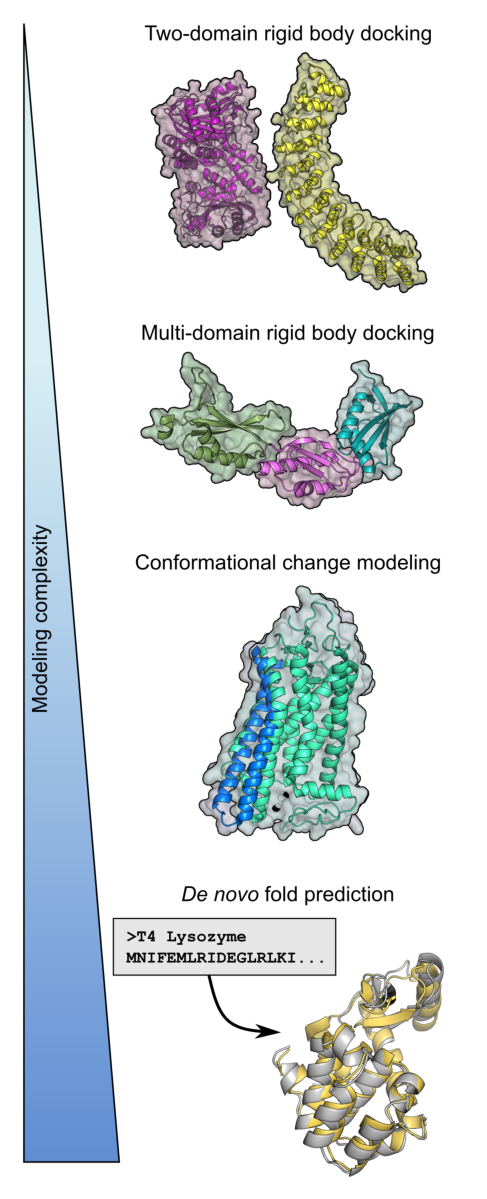
\includegraphics[width=2.5in]{deerintro_complexity.pdf}
 \caption[Protein modeling applications ranked by complexity.]{Protein modeling applications ranked by complexity. More complex problems, such as fold prediction or homology modeling, generally require more restraints to obtain accurate.}
\label{fig:deerintro_complexity}
\end{wrapfigure}

\section{Evaluating a model's agreement with experimental DEER data}

\subsection{Simulation of nitroxide side chains}\label{sec:deerintro_rotamers}

Accurately modeling a protein structure is only possible when the target conformation recapitulates the experimental data more effectively than alternative conformers. The reliance on flexible spin labels complicates the problem of identifying the conformer of interest using \gls{deer} data. Distances are measured between stably bound unpaired electrons far from the protein backbone; for example, in the widely used \gls{mtssl}, they are separated from the $\mathrm{C_{\upbeta}}$ atom by \SI{6}{\angstrom} and five $\upchi$ angles. Ultimately the linkers anchoring these unpaired electrons to the protein backbone determine how distances between unpaired electrons relate to distances between backbone atoms. Their conformations are generally not known in advance (although they can be determined using specialized algorithms, discussed in Section \ref{sec:deerintro_usingrawdata} below). Therefore, accurate models of protein structures require accurate distance distributions, which in turn require accurate predictions of spin labels rotamers.

However, the introduction of spin labels into the protein model is not straightforward. For example, several problems become apparent even in simple cases where protein structures being simulated in an MD environment are modified to have nitroxides at residues that have been experimentally labeled \citep*{Borovykh2006, Bowman2009, Brown2002, Corey2019, Hays2019, Islam2015, Islam2013, Marinelli2015, Marinelli2019, Roux2013}. First, whereas the two spin labels attached to any individual experimentally expressed double-cysteine mutant are unlikely to clash, an \emph{in silico} model attempting to integrate data from many \gls{deer} experiments may contain many explicitly modeled nitroxide side chains, some of which may be in close proximity to one another \citep*{Islam2013}. Second, the identity of the residue being labeled can provide valuable modeling information about which environments it preferentially occupies \citep*{Alexander2008}. For example, mutation of a tryptophan in a membrane protein to a nitroxide prevents it from informing the simulation software about structural characteristics such as membrane depth. Finally, and perhaps most critically, the computational cost of atomic-detail molecular dynamics simulations precludes its use as a screening tool that quantifies any given structural model's agreement with \gls{deer} data.

\Gls{mc} modeling paradigms provide one alternative approach. In this modeling paradigm, the spin label configurations are randomly picked from rotamer libraries, the probabilities of which are computed in advance. However, whereas rotamer statistics for canonical amino acids can be obtained directly from the PDB, those for nitroxide spin labels must instead be computed from detailed quantum mechanical calculations, a procedure described in detail elsewhere \citep*{Alexander2013, Edwards2014, Polyhach2011, Schmidt2015, Yang2020}. After obtaining these rotamers, \gls{mc} facilitates the rapid sampling a residue's local environment, and pairwise measurements can then be compared to experimental distances. The accuracy of distances obtained this way is comparable to those obtained by traditional \gls{md} \citep*{Klose2012} and in many cases are able to recover the rotamers observed experimentally \citep*{Alexander2013}. However, \gls{mc} methods have the advantage of being several orders of magnitude faster.

MDDS, an alternative developed by Islam and Roux, allows \gls{md} methods to rapidly calculate distance distributions from protein models in minutes to hours while avoid modeling spin labels to atomic detail \citep*{Islam2013}. By using a set of over fifty experimental distance restraints collected in T4 Lysozyme, they generalized the position of the unpaired electron with respect to the protein backbone. They then converted these positions into force fields between backbone atoms and a dummy atom representing the unpaired electron, allowing them to discard the rest of the nitroxide side chain.

\subsection{Simulation of DEER distance distributions}

Whereas experimental distance measurements are carried out between ensembles of molecules, computational methods generally model only a single structure at a time. To model the distribution of distance measured in ensembles of molecules, MDDS uses large numbers of noninteracting dummy atoms to build distance distributions \citep*{Kazmier2014a, Raghuraman2014}. Marinelli and Faraldo-Gomez instead used a time window to build their distributions from \gls{md} simulations between explicit nitroxide rotamers \citep*{Hustedt2018, Marinelli2015, Marinelli2019}. Alexander \emph{et al.} generated thousands of models using full-atom MC modeling and assembled distributions from those with the lowest energy \citep*{Alexander2013}.

By far the most common strategy in the literature models ensembles of possible nitroxide conformations. Methods such as MMM \citep*{Jeschke2018, Polyhach2011}, Pronox \citep*{Hatmal2012}, Nasnox \citep*{Beasley2015, Price2007, Tangprasertchai2015} and TagDock \citep*{Edwards2014} introduce every possible configuration stored in of a rotamer library one at a time and calculate Boltzmann energy values for those that do not clash with the rest of the protein. Some methods, such as TagDock, allow neighboring side chains to be repacked in response \citep*{Edwards2014}; others, such as MMM, can be applied to individual frames within an \gls{md} simulation to visualize the contribution of backbone dynamics \citep*{Stelzl2014, Tesei2020}. By contrast, MtsslWizard \citep*{Hagelueken2013, Hagelueken2012} uses \gls{mc} to sample rotamers until the number of either accepted rotamers or clashes reaches a predetermined threshold. A benchmark by Klose \emph{et al.} established that distributions simulated using these rotamer libraries are comparable in accuracy to those simulated using \gls{md}, with the distribution's average values deviating by about \SI{3.0}{\angstrom} from those observed experimental in each case \citep*{Klose2012}.

However, neither this approach, nor to our knowledge \gls{md}, can simulate distributions with widths that correlate with experimental values \citep*{Jeschke2013}, with the former consistently overstating spin label dynamics while neglecting backbone dynamics \citep*{Dastvan2016}. The only method that has achieved any correlation with experimental widths is a sampling-intensive \gls{mc} refinement approach that permits changes in the protein backbone \citep*{Alexander2013}, which suggests that coupling of backbone and side chain dynamics in solution may contribute to the width and shape of experimental distance distributions. Such a case has been crystallographically observed in the chaperone Spa15 when a loop containing a spin-labeled residue was found to slightly reconfigure compared to the wildtype structure \citep*{Lillington2011}.

One explanation for this discrepancy between experimental and simulated distribution widths is the fact that \gls{deer} measurements are almost always carried out in protein samples following the addition of cryoprotectants (such as glycerol) and flash-freezing. The common practice of submerging microliter-volume samples in liquid nitrogen gives spin labels up to hundreds of milliseconds to reconfigure and converge upon low-energy conformers \citep*{Schmidt2020}. Studies with T4 Lysozyme \citep*{Georgieva2012} and hemoglobin \citep*{Banham2007} have observed that the speed at which a sample freezes affects the width of the resulting experimental distribution. It is unclear if this effect could be corroborated \emph{in silico}, since the timescales of such a simulation are not currently feasible. Most likely, the experimental distribution likely involves a complex interplay between the spin label's local environment, the sample conditions and choices involved in its preparation, and the speed at which the sample was frozen.

\subsection{Scoring functions}\label{sec:deerintro_scoring_fxns}

How can the target conformation be identified if it cannot be expected to recreate the experimental data? Unfortunately, no consensus exists on this topic in the literature. Average values of distributions are widely used for the simple reason that their values correlate reasonably well with computational predictions made from structural models. As was just discussed, distribution widths cannot be recapitulated and are frequently ignored altogether, while distribution shapes are far more difficult to glean from the raw data and as a consequence rarely factor into modeling.

One strategy that has seen relatively widespread use is to model the nitroxide rotamers using a rotamer library such as MMM and to measure distances from the unpaired electron closest to the ensemble average \citep*{Dastvan2016, Duss2014, Duss2015, Duss2014a, Fehr2015, Raba2014, Ward2009}. Comparing these distance values to experimental averages allows a model to be scored using the sum of squared residuals. This retains the benefits of using the entire ensemble of spin label conformations while removing potentially unreliably information from the distance distribution. Nevertheless, alternative scoring functions sometimes are used that factor the width of the distribution. For example, in several studies, the deviation between the simulated and experimental average values has been divided by the experimental distribution's width. Presumably, this accounts for backbone heterogeneity by less aggressively penalizing deviations between residues with wider distributions \citep*{Jeschke2016, Peter2019}, although to our knowledge no benchmarks have been carried out to ascertain the merit of this fact. Alternatively, the entire shape can be retained, and the score of a model can be either its percent overlap \citep*{Hays2019, Jeschke2020, Kazmier2014a, Raghuraman2014} or the area between the integrals of the two distributions \citep*{Krug2016}.

It is important to note that regardless of the scoring function, the spin label's flexibility means that the direct application distance restraints to the unpaired electron or nitroxide bond to be largely ineffective at obtaining high-precision protein models, as the rotamers can easily reconfigure without any backbone changes. For example, when dummy atoms are used to model conformational changes modeled using MDDS, they have been found to absorb changes in the distance distribution, leaving the backbone untouched \citep*{Kazmier2014a, Raghuraman2014}. Applying distance restraints to the nitroxide bond of the rotamers in an MC simulation is fraught with similar challenges: for example, Herrick \emph{et al.} constrained the first two chi angles of \gls{mtssl} after finding that rotamers would otherwise adopt "unrealistic orientations" \citep*{Herrick2009, Lai2011}. Similar observations were made when modeling 5-NT \citep*{Krug2016} and Omp85 \citep*{Dastvan2016}. An exception is when data has also been collected using \gls{pre} paramagnetic relaxation enhancement \gls{nmr}, which measures distances between an unpaired electron and backbone nuclei. These distance data can be used as additional restraints on nitroxide rotamers to prevent them from reconfiguring \citep*{Milikisiyants2017, Saio2021, Wu2013}. However, the rotamers that contribute to the experimental signals may differ between the two datasets, since \gls{deer} samples are measured after flash-freezing whereas \gls{pre} samples are measured at room temperature.

\subsection{Limits of modeling protein structures using explicitly modeled rotamers and rotamer libraries}

Distance distributions in non-\gls{md} environments can typically be simulated in seconds or tenths of a second, with the majority of computation time typically devoted to calculating clashes with the rest of the protein. Unfortunately, even these speeds still preclude the use many modeling applications. Most studies therefore use these methods to screen models \emph{ex post facto}, rather than restrain them directly during sampling. Some studies circumvent these cost restrictions by introducing rotamers prior to modeling and retaining them throughout sampling without recalculating clashes, thus skipping the most computationally expensive step. Such a strategy was appropriate when docking CDB3 and Ankyrin \citep*{Edwards2014}, as the local environment of the spin labels were not expected to change throughout the docking simulation. Alternatively, a number of studies only retain the rotamer closest to the center of the ensemble: by fixing it in space relative to the backbone, it could be restrained using distance data without risking its reconfiguration \citep*{Bibow2017, Duss2014, Duss2014a, Raba2014,  Ward2009}.

\subsection{Direct integration of DEER data during sampling using restraints between backbone atoms}\label{sec:deerintro_main_integration}

Because of this computational cost issue, these data are more frequently integrated as restraints between backbone atoms during sampling. Restraints between $\mathrm{C_{\upbeta}}$ atoms are more common, although $\mathrm{C_{\upalpha}}$ atoms have also been used \citep*{Park2006, Sale2004}. While trivial to implement in most modeling packages, this approach requires that distance values between spin labels be transformed into distance restraints between backbone atoms. Unfortunately, these measurements do not always line up perfectly \citep*{Hirst2011}. Yang \emph{et al.} demonstrated the danger of taking these experimental distances at face value when predicting the structure of the homodimer Dsy0195 \citep*{Yang2010}. The \gls{rmsd} of their model improved when using a restraint with an experimental \gls{deer} distance that matched the $\mathrm{C_{\upbeta}}$-$\mathrm{C_{\upbeta}}$ distance, but worsened when the two values differed by as little as \SI{5}{\angstrom}. As has been previously noted \citep*{Alexander2008, Bhatnagar2007, Borbat2002, Fischer2016, Georgieva2013, Jeschke2013, Sale2005}, deviations of this magnitude are not uncommon. In globular proteins, spin labels tend to face away from each other, leading to experimental distances values that exceed the corresponding $\mathrm{C_{\upbeta}}$-$\mathrm{C_{\upbeta}}$ distance by a median of \SIrange{6}{7}{\angstrom}. By contrast, the deviations between these values across protein-protein interfaces are lower but nonetheless significant \citep*{Bhatnagar2007, Fischer2016, Kim2011}. Notably, these values exceed the \SI{3}{\angstrom} deviation observed between the average values of simulated and experimental \gls{deer} distance distributions, highlighting the loss of precision that comes with this scoring approach \citep*{Sale2005}.

Backbone potentials frequently score a model's agreement with experimental data using wide and flat-bottomed harmonic potentials. These have be introduced as NOE-like restraints into programs such as CYANA \citep*{Guentert2004}, Xplor-NIH \citep*{Schwieters2003}, CNS \citep*{Brunger1998}, Rosetta \citep*{Leaver-fay2011, Leman2020, Simons1997}, and BCL \citep*{Karakas2012, Woetzel2012}. Both Alexander \emph{et al.} and MacCallum \emph{et al.} successfully predicted the structures of T4 Lysozyme and aA-crystallin \emph{de novo} using this type of restraint \citep*{Alexander2008, MacCallum2015}. In both cases, a score of zero was assigned to $\mathrm{C_{\upbeta}}$-$\mathrm{C_{\upbeta}}$ distances (in angstroms) ranging from $\upmu_\mathit{SL} - \upsigma_\mathit{SL} - 12.5$ to  $\upmu_\mathit{SL} + \upsigma_\mathit{SL} + 2.5$, where $\upmu_\mathit{SL}$ and $\upsigma_\mathit{SL}$ are the average values and standard deviations of the experimental distribution. Similarly, Kim \emph{et al.} determined the docking interface of CDB3 and Ankyrin using a criterion in which any model was kept if its $\mathrm{C_{\upbeta}}$-$\mathrm{C_{\upbeta}}$ distances deviated by less than \SI{14}{\angstrom} from the experimental average distance \citep*{Kim2011}. Alternatively, the edges of the distribution have been used as restraints bounds \citep*{Bibow2017}.

These scoring functions, although broad, can nonetheless respond poorly to outliers. Bhatnagar \emph{et al.} noted when docking CheA and CheW that a pair of $\mathrm{C_{\upbeta}}$-$\mathrm{C_{\upbeta}}$ restraints whose distance deviated substantially from experimental interspin distance values prevented low-\gls{rmsd} models from being obtained; their removal improved the \gls{rmsd} of the docking interface from over \SI{10}{\angstrom} to \SI{2.6}{\angstrom} \citep*{Bhatnagar2007}. However, they used a more restrictive potential with lower and upper bounds of $\upmu_\mathit{SL} -$\SI{5.0}{\angstrom} and $\upmu_\mathit{SL} +$\SI{1.0}{\angstrom}, respectively, which may increase the scoring function's sensitivity to outliers \citep*{Bhatnagar2010}.

A similar strategy was employed by Evans \emph{et al.} when modeling conformational changes in the ion channel SthK \citep*{Evans2020}. They took advantage of a starting conformation, as well as a set of \gls{deer} data for that conformation, by applying the magnitude of the distance change as a harmonic restraint between $\mathrm{C_{\upbeta}}$ atoms with a lower and upper bound of $\upmu_\mathit{SL} -$\SI{1.0}{\angstrom} and $\upmu_\mathit{SL} -$\SI{1.0}{\angstrom}, respectively. This strategy has the benefit of reducing variation among generated models but assumes that domains and spin labels do not rotate or substantially reconfigure with respect to one another.

Hirst \emph{et al.} generated a custom cubic spline function called the \gls{cone} model that, unlike a flat-bottomed harmonic function, accounts for the fact that the experimental distance is more likely, but not necessarily guaranteed, to be longer than the $\mathrm{C_{\upbeta}}$-$\mathrm{C_{\upbeta}}$ distance \citep*{Hirst2011}. Its use improved the number of high-resolution models folded \emph{de novo} for T4 Lysozyme, and it has since been applied to problems involving \emph{de novo} folding \citep*{Fischer2015, Fischer2017, Fischer2016}, docking \citep*{Alexander2014, Dastvan2016, Fischer2016, Tessmer2018}, and conformational change modeling \citep*{Dastvan2016, Kim2012, Krug2016, VanEps2011}.

None of these approaches can determine unequivocally the structures of proteins or complexes. For example, Kim \emph{et al.} found that the incorporation of twenty experimental restraints when docking CDB3 and Ankyrin led to a wide range of possible configurations \citep*{Kim2011}. This highlights the breadth of the solution space, even in cases where the experimental restraints outnumber the degrees of freedom by more than threefold. Ultimately this pool of models was further trimmed using an orthogonal set of \gls{epr} data that measured the solvent accessibility of individual spin-labeled residues.

This hierarchical approach contrasts with the direct integration of flat-bottomed harmonic restraints into sampling, which has the intended effect of directing the modeling protocol to a conformational subspace encompassing the target structure. Optimization within this subspace proceeds using additional criteria, such as energy functions or experimental \gls{nmr} restraints, which can evaluate structural features with greater precision. The MELD structure prediction program, for example, navigates this subspace using AMBER forcefields and replica exchange molecular dynamics \citep*{MacCallum2015, Perez2016}, whereas Rosetta relies on its coarse-grained energy function and \gls{mc} sampling \citep*{Alexander2008, Kazmier2011}. By contrast, Ling \emph{et al.} used Xplor-NIH to model the structure of YagP by combining \gls{deer} data with \gls{epr} membrane depth restraints \citep*{Ling2016}. In each case, the flat-bottomed potentials do not interfere with optimization within this region; instead, they guide the conformational search away from false minima that fall outside their bounds. As a result, the weights of these restraints, relative to other experimental restraints or score terms, is not generally optimized or fine-tuned. 

By contrast, the \gls{cone} model developed by Hirst \emph{et al.} does introduce a bias into the search procedure by assuming that the experimental distance will usually, but not always, exceed the $\mathrm{C_{\upbeta}}$ distance. This assumption modifies the function landscape and must therefore be carefully integrated into the modeling protocol. During the development of this energy potential, Hirst \emph{et al.} determined by grid search a weight for this energy potential that maximized the proportion of high-accuracy models of T4 Lysozyme. This weight has since been used in virtually all cases outlined above.

We note that although these restraints are imprecise, they are often followed by the use of higher-precision scoring functions in conjunction with atomic-detail depictions of spin label rotamers more amenable to the identification of accurate models \citep*{Sarver2018}. For example, structural modeling of EmrE was achieved using the \gls{cone} model in BCL::Fold followed by refinement with Modeller using the rotamer libraries available in MMM \citep*{Dastvan2016}. The structure of the C-terminus of ExoU was similarly modeled \emph{de novo} using the \gls{cone} model, followed by \emph{in silico} spin labeling with explicit \gls{mtssl} side chains using Rosetta \citep*{Fischer2017}. The CheA/CheW binding interface was determined by generating a set of initial models using $\mathrm{C_{\upbeta}}$-$\mathrm{C_{\upbeta}}$ restraints followed by finer-grain selection using rotamer libraries \citep*{Bhatnagar2007}. Thus, the use of coarse backbone restraints can set the stage for finer-grain modeling.

\subsection{Error analysis}

Our discussion has extensively mentioned the limit of \gls{deer} restraints in modeling structures: even docking interfaces cannot be determined with absolute certainty using these data. Fortunately, quantification of the uncertainty of these models is increasingly widely used. Cross-validation requires that multiple subsets of these restraints be used for modeling, and the results compared to check the stability of the solutions. This approach has been used to model the NhaA homodimer \citep*{Hilger2007}, 5-NT \citep*{Krug2016}, and RmsE/RmsZ \citep*{Bhatnagar2007}. The docking interface of the NhaA homodimer, for example, was determined using each of the 36 available combinations of seven restraints from nine restraints available, leading to an \gls{rmsd} of \SI{0.45}{\angstrom} among each of the thirty-six best models from each set \citep*{Hilger2007}. Bowen and colleagues took this idea a step further and quantified the uncertainty resulting from the choice of rotamer library \citep*{Bowen2018}. Alternatively, if a starting structure is available, the error calculated for that structure can be used to inform the precision with which certain features and/or substructures of a protein can be modeled with high confidence. Bliecken \emph{et al.} calculated the deviations among restraints in the soluble Bax monomer, which had been initially determined using \gls{nmr}, and used those values to inform the accuracy of their model for the membrane-bound Bax dimer \citep*{Bleicken2014}. More commonly, uncertainty is depicted informally, for example by presenting a handful of the best-scoring models \citep*{Evans2020, Gigli2018, Kim2011}. Far more often it is ignored altogether.

\subsection{Integrating DEER restraints with other types of experimental data}

Flat-bottomed harmonic functions, although imprecise, nonetheless allow DEER data to be elegantly integrated into a modeling protocol involving other types of data. When modeling distributions using programs such as MMM, it is less clear how best to jointly consider agreement with both \gls{deer} data and, for example, \gls{saxs} data. One option mentioned above is to use hierarchical approaches, where models are effectively filtered out if they fail to satisfy each of several experimental criteria. Bowman, Boura, and Sundaramoorthy combined \gls{deer} and \gls{saxs} data using this approach for rigid-body modeling of Vps75/Nap1, ECSRT-I, and Chd1, respectively \citep*{Boura2012, Boura2011, Bowen2018, Sundaramoorthy2017}. In each case, models needed to be docked in such a way that both the \gls{deer} data and \gls{saxs} density were satisfied. Several examples in the literature exist in which this is done informally, such that a solution obtained using \gls{deer} data is simply validated using experimental data from another source. Hilger \emph{et al.} compared their model for the dimeric NhaA antiporter to previously published low-resolution 2-D cryo-electron microscopy data \citep*{Hilger2007}, whereas Sung \emph{et al.} docked their model of Bax into \gls{saxs} density \citep*{Sung2015}.

A preferable approach is the direct integration of the two during sampling. This, however, requires that scores be balanced in such a way that avoid overemphasizing data from either method. To our knowledge, no single widely used approach exists. In the literature, ESCRT-II was modeled using both \gls{saxs} and \gls{deer} data using a $\chi^2$ potential for each experimental technique \citep*{Boura2012}. Peter \emph{et al.} also used $\chi^2$ potentials to model YopO using both \gls{saxs} and \gls{deer}, but simply compared the average values of the simulated and experimental distributions \citep*{Peter2019}.

\subsection{When simulation guides experiment: choosing restraints using starting structures}

Several application-specific algorithms have been developed that recommend experimental restraints. These recommendations are typically application-specific, as the demands of each application change the information being sought by the experimental data. As an example, \emph{de novo} folding problems benefit from restraints between residues that are distant in sequence but close in space. The \gls{mc} algorithm developed by Kazmier \emph{et al.} that chooses restraints for \emph{de novo} folding uses two criteria: it tries to ensure that the pairs of residues are far apart in sequence space while diversifying their placements to avoid collecting redundant information, for example between the same pair of helices \citep*{Kazmier2011}. By contrast, when a structure is known but its loops are not, networks of four restraints per spin-labeled loop residue have been proposed in a procedure analogous to triangulation \citep*{Jeschke2016}. For conformational change problems, both Hays \emph{et al.} \citep*{Hays2018} and Mittal and Shukla \citep*{Mittal2017} developed restraint-picking methods for conformational change modeling problems that prioritize the reduction of redundant information by selecting residue pairs whose movements are minimally correlated; both rely on short nanosecond \gls{md} simulations to obtain an initial guess for these structural dynamics. If for some reason such a simulation is impossible, an alternative method \citep*{Jeschke2012a} predicts which regions of a protein structure will move using normal mode analysis and a modification of the Zheng-Brooks algorithm \citep*{Zheng2005}. The same author proposed a separate criterion for rigid body docking problems, which require far fewer restraints to define analytically \citep*{Jeschke2020}. Since only three residues need to be spin labeled per rigid body, an intuitive choice is to choose the three residues in each rigid body that generate the largest nearly-equilateral triangle. This minimizes the propagation of errors throughout the docked structure.

\section{Towards the analysis of DEER data by structural modeling}\label{sec:deerintro_usingrawdata}

The first half of this chapter discussed the difficulty of extracting distance data from \gls{deer} traces in the time domain, while the second half discussed how best to use those distance data for modeling protein structures. In principle, the two steps can be directly integrated by attempting the simulate the raw data using the same approach summarized earlier. Briefly, the conformation determines the distance distributions being fitted and reconfigures to improve the goodness-of-fit in the time domain. Several studies have attempted to recapitulate the raw data from protein models as early as 2007 \citep*{Bhatnagar2007, Hilger2007}. The previously mentioned ESCRT-II, which was modeled using the raw \gls{deer} traces alongside \gls{saxs} data using a $\chi^2$ potential to balance the two \citep*{Boura2012, Boura2011}. Marinelli and Fiorin modeled a conformational change in VcSiaP by restraining the spin labels directly using the raw data \citep*{Marinelli2019}. Notably, both the study of VcSiaP and NhaA also attempted to fit the background contribution to the signal, which was added to the simulated data using a "fit-within-a-fit" procedure. By contrast, the study of ESCRT-II, as with others \citep*{Reichel2018}, background-corrected the data before using it as a restraint.

Additionally, we mentioned in this chapter that native or correctly folded models are not expected to perfectly recapitulate the experimental \gls{deer} distance distribution. Failure to account for this expectation can cause the data to be overfitted. In fact, whereas this expectation can easily be encoded into the scoring function when scoring models using data in the distance domain - for example, using broad, flat-bottomed functions (see Section \ref{sec:deerintro_scoring_fxns} above) - it is far more difficult to anticipate the magnitude of these deviations in the time domain. This imprecision prevents minor contributions to the experimental signal from being resolved, removing one of the fundamental advantages of the \gls{deer} technique.

How can this issue be addressed? One might intuit that less flexible spin labels, the positions of which can more precisely be simulated from the backbone, may be positioned to improve the precision of simulated distributions enough to permit modeling using data in the time domain. Several options are explored in the literature. The label IDSL (also called V1 or RSSR), for example, has far less rotameric freedom than \gls{mtssl} and leads to sharper distance distributions \citep*{Balo2016, Warshaviak2013}. Other alternatives that have been used for modeling include bifunctional spin labels \citep*{Fajer2015, Islam2015, Sahu2017} and paramagnetic copper ions \citep*{Cunningham2015, Merz2014} that are conjugated to or coordinated by pairs of alpha carbons. By reducing or altogether eliminating the contribution of rotamer dynamics to the width of the distribution, these methods can potentially isolate the contribution of backbone dynamics. Moreover, it avoids the risk of uncritical accepting the width of the rotamer distribution obtained from methods such as MMM, which may cause backbone dynamics to be understated (see Section \ref{sec:deerintro_rotamers}).

A second option to reduce uncertainty is to determine the positions of flexible spin labels in advance. This triangulation procedure, however, requires a conformation of the protein to be known \emph{a priori} that is consistent with a set of experimental data. The positions of the spin labels can be determined by singular value decomposition  \citep*{Hagelueken2013}, non-linear least squares minimization \citep*{Bleicken2014}, or by eye \citep*{Wingler2019}. An instructive example is provided in the study of the Angiotensin receptor, where distance distributions attributed to a known conformation were used to determine which rotamers were sampled in solution\citep*{Wingler2019}. The distance data from other conformations were then used for conformational change modeling using \gls{md}. Similarly, the model of dimeric membrane-embedded Bax was obtained by first determining the \gls{mtssl} rotamers from the monomeric model \citep*{Bleicken2014}. However, the constraints placed upon rotamer triangulation - that a conformation is both known to high resolution and consistent with a set of experimental data - make it uncommon, and this technique has not yet been used to model proteins using data in the time domain. More often, it is used to localize a paramagnetic ligand or ion within the same structure \citep*{Gaffney2012, Yang2012}.

What would the key benefit be of working with the raw data? To answer this question, it may be prudent to take a global perspective on the state of the art, as outlined in Section \ref{sec:deerintro_deeranalysis} above. \Gls{deer} data are commonly background corrected, then analyzed; \gls{deer} distance distributions are partitioned among several conformations, with the average peak of each component frequently isolated for the purposes of modeling. As discussed above, information lost during each of these four steps cannot later be recovered. It may, however, be accessible to one-step approaches that simulating the raw data from an ensemble of models. It is in precisely this direction that we hope the field moves.